\begin{figure}[h!]
    \centering
    \caption{Distribution of changes in minimum wage measures under a 
             counterfactual federal minimum wage of \$9, urban ZIP codes}
    \label{fig:cf_hist_res_and_wkp_mw}
    
    \begin{subfigure}{0.5\textwidth}
        \caption*{Residence MW}
        \includegraphics[width = 1\textwidth]{counterfactuals/output/hist_d_mw_res_fed_9usd}
    \end{subfigure}%
    \begin{subfigure}{0.5\textwidth}
        \caption*{Workplace MW}
        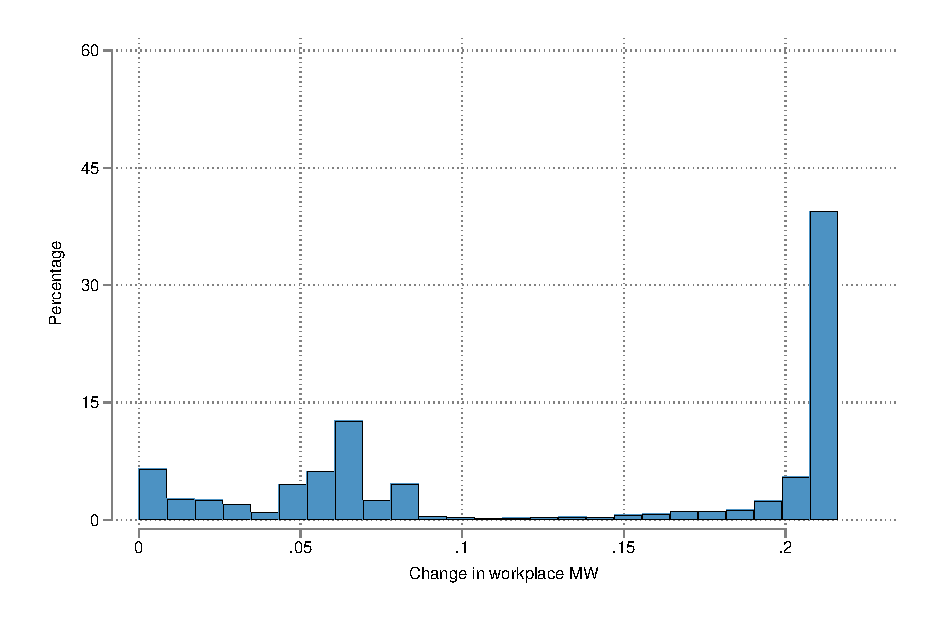
\includegraphics[width = 1\textwidth]{counterfactuals/output/hist_d_mw_wkp_fed_9usd}
    \end{subfigure}

    \begin{minipage}{.95\textwidth} \footnotesize
        \vspace{3mm}
        Notes:
        Data are from LODES and the MW panel described in Section
        \ref{sec:data_mw_panel}.
        The figures show the distribution of changes in the residence and 
        workplace MW measures generated by a counterfactual increase to \$9 
        in the federal MW in January 2020, holding constant other MW policies 
        in their December 2019 levels.
        The unit of observation is the urban ZIP code, where we define a ZIP code 
        as urban if it belongs to a CBSA with at least 80\% of its population 
        classified as urban by the 2010 Census.
    \end{minipage}
\end{figure}
